%%%%%%%%%%%%%%%%%%%%%%%%%%%%%%%%%%%%%%%%%%%%%%%%%%%%%%%%%%%%%%%%%%%%%%%%
% Plantilla TFG/TFM
% Escuela Politécnica Superior de la Universidad de Alicante
% Realizado por: Jose Manuel Requena Plens
% Contacto: info@jmrplens.com / Telegram:@jmrplens
%%%%%%%%%%%%%%%%%%%%%%%%%%%%%%%%%%%%%%%%%%%%%%%%%%%%%%%%%%%%%%%%%%%%%%%%

\chapter{Resultados}
\label{resultados}
\section{Método por parcelas}
\subsection{Optimización}
\par La optimización de los datos de entrada tiene su base en la elección de los sets de parcelas de entrenamiento y test, siendo los mejores resultados para todos los casos el uso de un conjunto de 6 parcelas para entrenamiento y 1 para la evaluación. En cuanto a la optimización del regresor, se basa en la determinación del número de árboles que lo componen. La relación entre el número de árboles para un modelo y el coeficiente de determinación es un buen descriptor para la elección de este parámetro, como se presenta en la imagen de ejemplo \ref{fig:opt_parcl} con el caso de salida \gls{bbch}. En ella, se puede ver que una vez alcanzado cierto nivel de coeficiente, la mejora de este en relación al aumento del número de árboles no es significativa con respecto al costo computacional y a la complejidad del sistema que se crea. 
\begin{figure}[h]
    \centering
    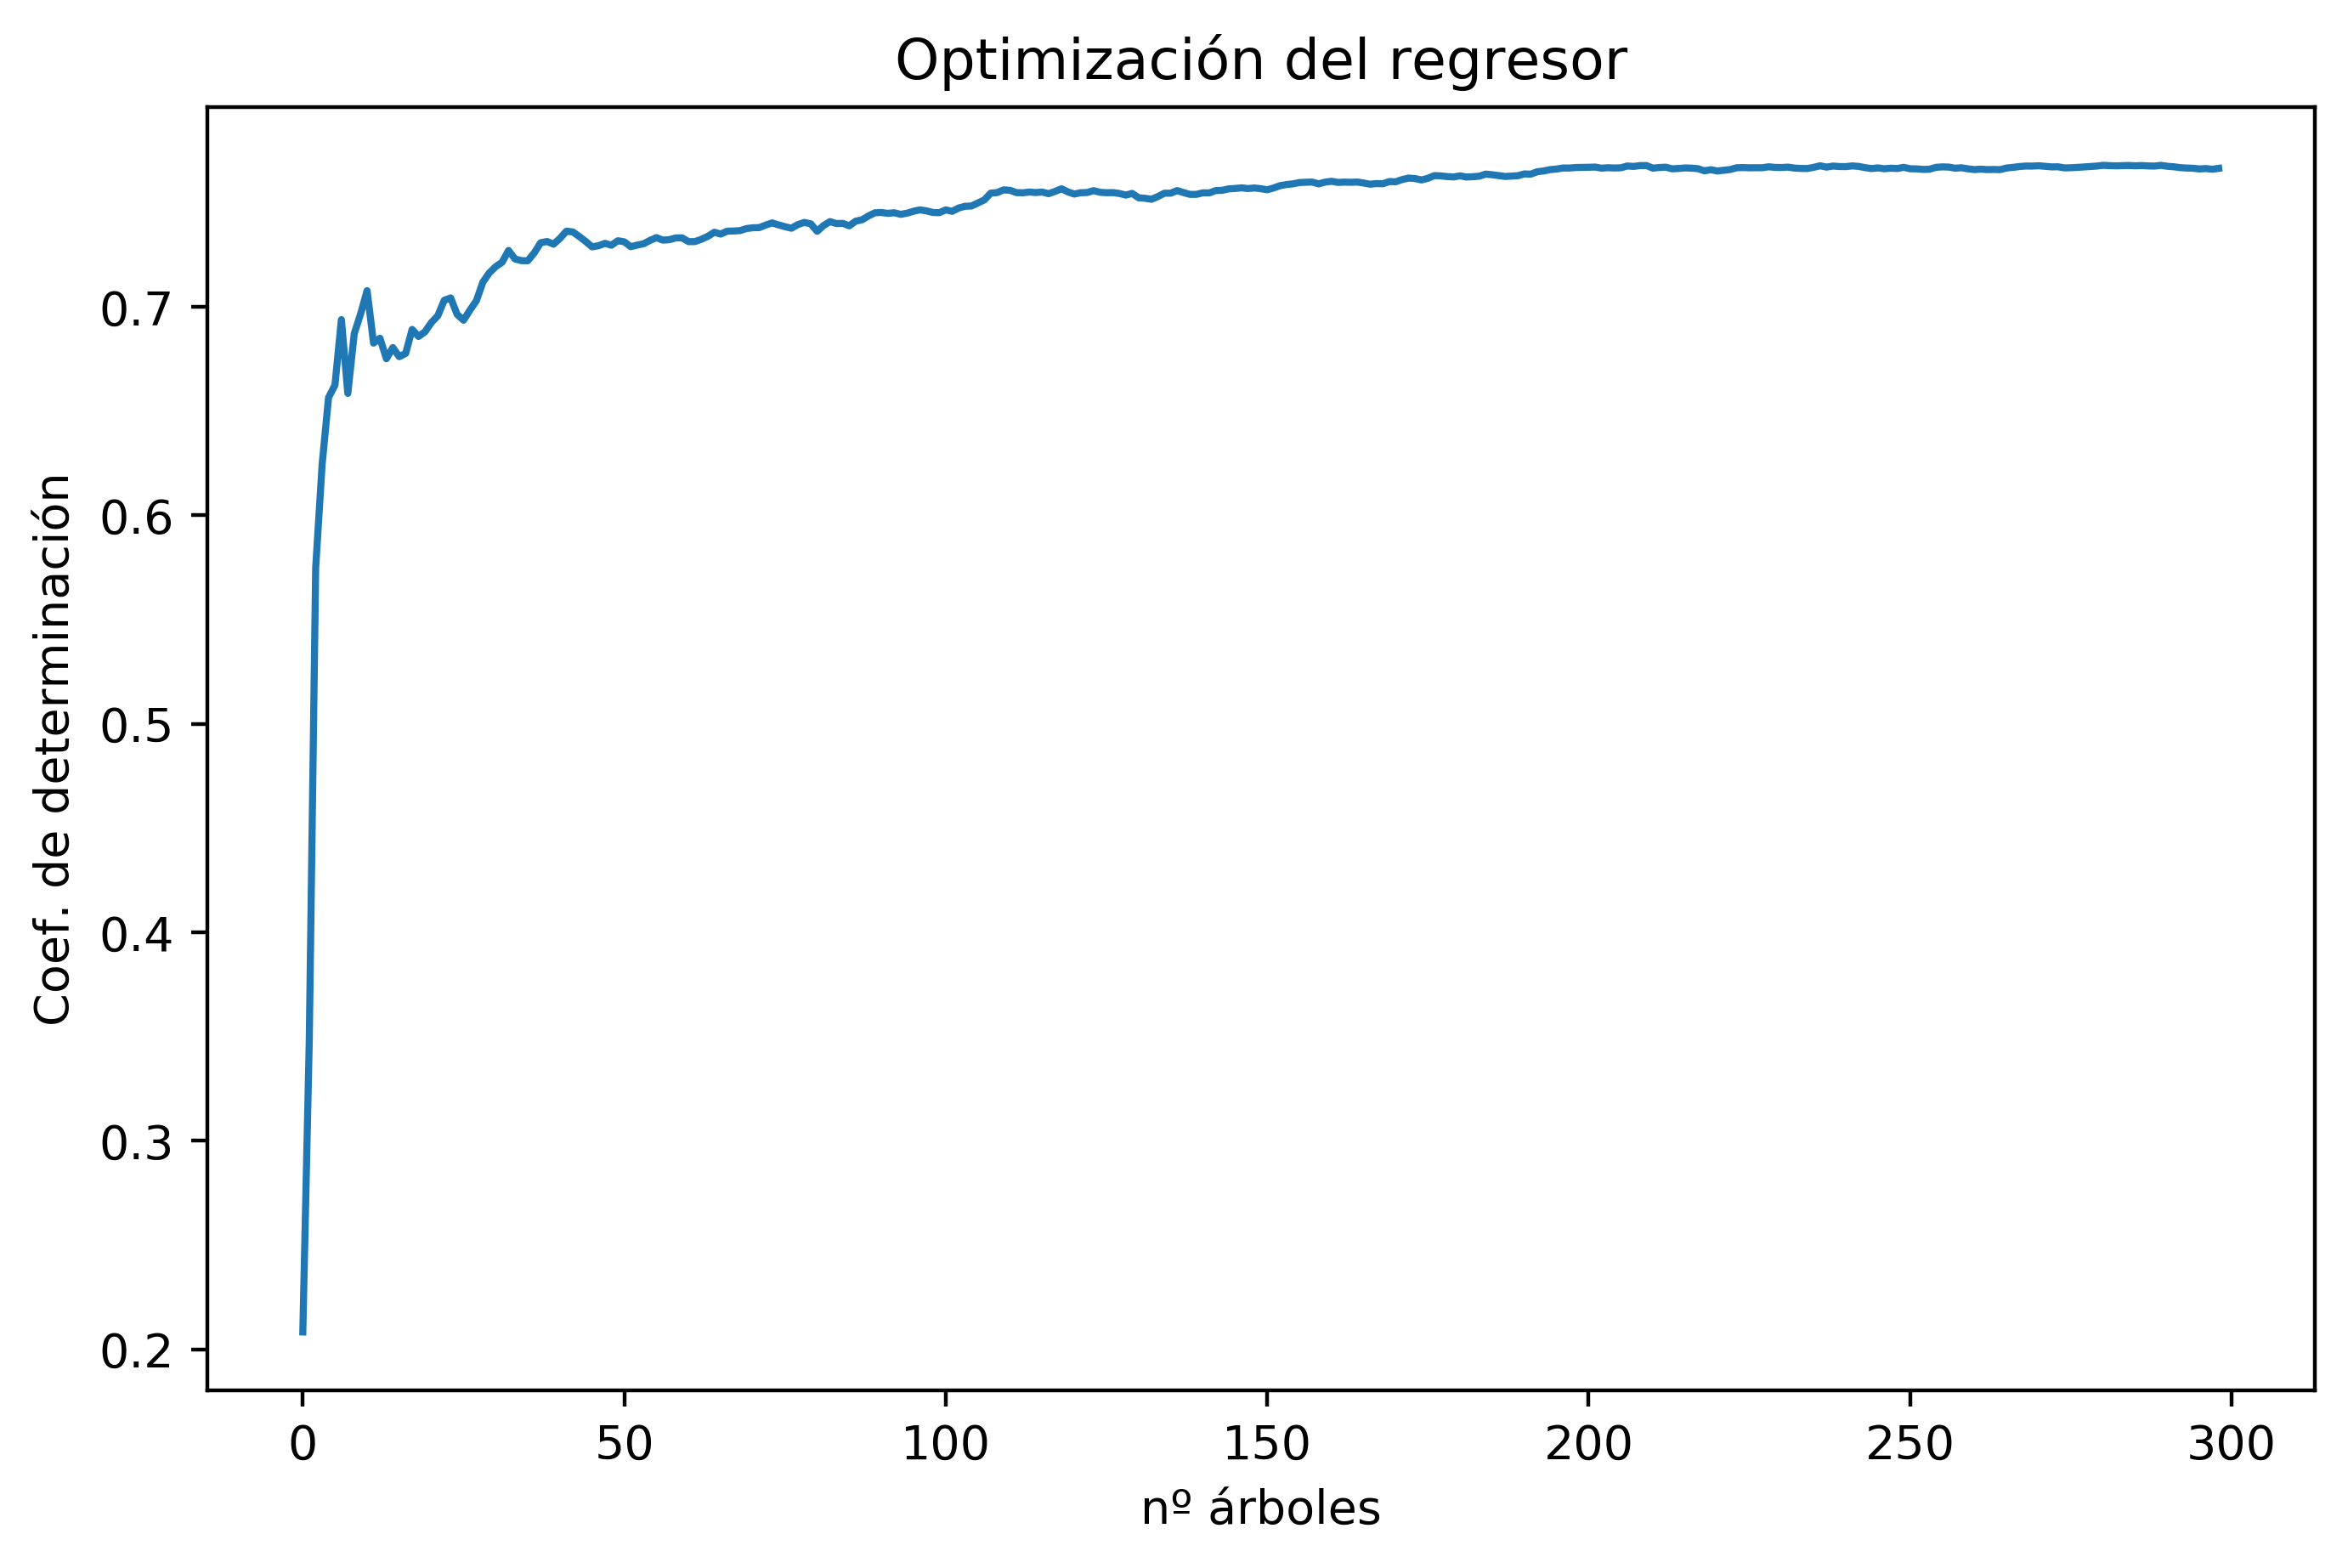
\includegraphics[height=9cm]{archivos/tfg/opt_tree_bbch_mean} 
    \caption{Optimización del número de árboles para \gls{rfr} en el modelo de salida \gls{bbch}\label{fig:opt_parcl}}
    
\end{figure}

\par Finalmente, los parámetros utilizados en este método para cada caso se presentan en la tabla \ref{tab:opt_parcl}, donde se pueden ver: la parcela utilizada para el periodo de test del modelo; siendo el resto de parcelas utilizadas en el entrenamiento, y el número de árboles óptimo para \gls{rfr}, de acuerdo con la evolución del coeficiente de determinación para cada caso.

\begin{table}[h]
\centering
\begin{tabular}{l|ccc}
                  & BBCH     & Altura   & BBCH\&Altura \\ \hline
Parcela de test   & `Mínima' & `Puntal' & `Mínima'     \\
Número de árboles & 42       & 77       & 54          
\end{tabular}
\caption{Parámetros de optimización de entrada y modelo
\label{tab:opt_parcl}}
\end{table}

\par Como se puede observar, los 3 casos de este método constan de un número óptimo de árboles de, al menos, el mismo orden. Cabe destacar que el aumento de complejidad en el modelo, sobre todo en el caso de la altura como salida del sistema.  
\subsection{Salidas del modelo}
\subsection{Evaluación}
\section{Método por píxeles} 
\subsection{Optimización}
\par La optimización de los datos de entrada para este método se realiza de igual manera que el anterior, coincidiendo los mejores resultados para todos los casos en el uso de un conjunto de 6 parcelas para entrenamiento y 1 para la evaluación. En cuanto a la optimización del regresor, se utiliza también la relación entre el número de árboles para un modelo y el coeficiente de determinación, presentado en la imagen de ejemplo \ref{fig:opt_pixl} con el caso de salida \gls{bbch}. En ella, se puede ver que una vez alcanzado cierto nivel de coeficiente, la mejora de este en relación al aumento del número de árboles no es significativa con respecto al costo computacional y a la complejidad del sistema que se crea. 
\begin{figure}[h]
    \centering
    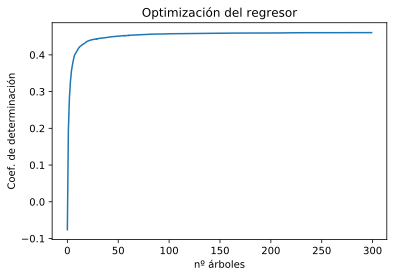
\includegraphics[height=9cm]{archivos/tfg/opt_tree_bbch_pixel} 
    \caption{Optimización del número de árboles para \gls{rfr} en el modelo de salida \gls{bbch}}
    \label{fig:opt_pixl}
\end{figure}

\par Finalmente, los parámetros utilizados en este método para cada caso se presentan en la tabla \ref{tab:opt_pixl}, donde se pueden ver: la parcela utilizada para el periodo de test del modelo; siendo el resto de parcelas utilizadas en el entrenamiento, y el número de árboles óptimo para \gls{rfr}, de acuerdo con la evolución del coeficiente de determinación para cada caso.

\begin{table}[h]
\centering
\begin{tabular}{l|ccc}
                  & BBCH     & Altura   & BBCH\&Altura \\ \hline
Parcela de test   & `Mínima' & `Mínima' & `Mínima'     \\
Número de árboles & 46       & 48       & 47          
\end{tabular}
\caption{Parámetros de optimización de entrada y modelo \label{tab:opt_pixl}}
\end{table}

\par Como se puede observar, los 3 casos coinciden en el set de parcelas de entrenamiento y test con el que se obtienen mejores resultados. Probablemente esto se debe a anomalías en el desarrollo de algunas parcelas, las cuales, si se toman como set de test, el modelo no las habría podido tener en cuenta en el aprendizaje y el error en la predicción sería mayor. Los 3 casos de este método constan de un número óptimo de árboles muy similares, con una diferencia de 1 y 2 con respecto al caso menor. Cabe destacar que el aumento de complejidad, aunque escaso, en el modelo de salida de la altura, como ocurre para el método anterior. Además, tanto para la metodología por píxeles como por parcelas, se obtiene un número óptimo de árboles para el caso de 2 salidas intermedio a los óptimos para las mismas salidas en modelos independientes. Esto se debe a una compensación en la estimación de ambas variables, para que una variable sea óptima sin que su mejora sea a costa de la otra se llega a un valor intermedio en el que ninguna de las salidas está totalmente optimizada pero tienen el mejor resultado del sistema compartido completo. 


\subsection{Salidas del modelo}
\subsection{Evaluación}
%%%%%%%%%%%%%%%%%%%%%%%%%%%%%%%%%%%%%%%%%%%
%%%%%%%%%%%%%%%%%%%%%%%%%%%%%%%%%%%%%%%%%%%
\section{Comparativa de métodos}
\par La evaluación general de resultados realizada es la comparación entre los dos métodos de procesamiento de datos de entrada mencionados: a nivel de parcela o de pixel. En las siguientes tablas se pueden ver la evaluación de los resultados, divididos en entradas a nivel de parcela ~\ref{tab:errorpc} y a nivel de pixel ~\ref{tab:errorpx}, según los índices estadísticos de \gls{mae}, \gls{rmse} y el coeficiente de determinación ($R^2$). Ambos conjuntos corresponden al mejor caso de cada método, esto es, habiendo seleccionado sus parámetros de entrada óptimos en cuanto a número de variables y set de parcelas de entrenamiento, y habiendo optimizado también los parámetros del regresor.

\begin{table}[h]
\centering
\begin{tabular}{lccc}
\multicolumn{4}{c}{Datos de entrada a nivel de parcela}                            \\ \hline \hline
\multicolumn{1}{l|}{}                            & BBCH  & Altura & BBCH\&Altura \\ \cline{2-4} 
\multicolumn{1}{l|}{$R^2$}                       & 0.74  & 0.65   & 0.70 \\
\multicolumn{1}{l|}{\gls{rmse}} 				 & 15.39 & 17.87  & 15.69 \\
\multicolumn{1}{l|}{\gls{mae}}  				 & 11.13 & 14.21  & 12.63       
\end{tabular}
\caption{Índices estadísticos de las predicciones con datos de entrada a nivel de parcela. \label{tab:errorpc}}
\end{table}

\begin{table}[h]
\centering
\begin{tabular}{lccc}
\multicolumn{4}{c}{Datos de entrada a nivel de pixel}                            \\ \hline \hline
\multicolumn{1}{l|}{}                            & BBCH  & Altura & BBCH\&Altura \\ \cline{2-4} 
\multicolumn{1}{l|}{$R^2$}                       & 0.45  & 0.52   & 0.45         \\
\multicolumn{1}{l|}{\gls{rmse}} 				 & 22.23 & 19.89  & 21.17        \\
\multicolumn{1}{l|}{\gls{mae}}  				 & 17.26 & 15.64  & 16.58       
\end{tabular}
\caption{Índices estadísticos de las predicciones con datos de entrada a nivel de pixel.\label{tab:errorpx}}
\end{table}

\par Como se puede observar, para las 3 posibles salidas para las que se han diseñado los modelos, el método que emplea datos de entrada a nivel de parcela consigue notablemente mejores resultados. Se obtienen valores de coeficiente de determinación más cercanos a 1, valor ideal, apreciándose en el modelo de predicción de \gls{bbch} una mejora para el caso de parcelas de un 64.4\% con respecto al de pixel. Lo mismo ocurre en los índices de error, cuyo valor óptimo es 0: se obtienen valores inferiores para el método a nivel de parcela en todos los casos estudiados.
\\
\par Los mejores resultados obtenidos para el procesamiento a nivel de parcelas pueden recaer en que todos los datos recogidos de verdad de tierra se presentan por parcelas, por lo que no existen unos datos para contrastar cada pixel extraído de la información de satélite con el terreno. Dentro de cada parcela el cultivo no tiene porqué desarrollarse de manera homogénea, pero la información recibida de este consta del valor de \gls{bbch} (con el requisito de ser el correcto para al menos el 50\% del cultivo) y la altura generalizados por parcela, además de los máximos y mínimos de cada uno, por lo que las variaciones que se puede hallar en distintas zonas del cultivo no se tienen en cuenta. Por ello, el método de pixel implementado asigna un solo valor de salida para conjuntos de píxeles de la misma parcela, los cuales pueden estar representando unos niveles de \gls{bbch} o altura distintos, y esto conlleva un ajuste del modelo erróneo y, por tanto, peores índices estadísticos de evaluación. Aún así, este método no ha sido descartado, ya que el análisis a nivel de pixel es de gran interés para detectar esas variaciones de desarrollo de un cultivo dentro de una misma parcela. 